\chapter{Background} %concepts
\label{chap:background}
% Just description of fundamental concepts in which the thesis is built upon. Do not need to list all concepts, but only major ones.
    The following chapter supplies an overview of the fundamental concepts that this thesis is based upon. As a first step, \textit{Neurobiology} is considered as many other topics require a basic understanding of our nervous system. Therefore its most important structures and their functionality are explained. Based on this, \textit{Cognitive Processes} are considered. A focus is thereby laid upon some examples that are of particular interest to this thesis.
    But also, the concept of \textit{Cognitive warfare} is being explored. First supplying a general overview of this rather broad field, followed by a more detailed analysis of NeuroStrikes and their relevance.
    Subsequently, \textit{Brain-Computer Interfaces} and their technological underpinnings are discussed. By presenting a few examples of both invasive and non-invasive methods, their capabilities and potential use cases are revealed.
    Finally, the topic of \textit{Brain Simulations} is introduced and some prominent examples of simulators are discussed, revealing their differences and specific use cases. 


\section{Neurobiology}
    %Overview of the Neurobiological part and relevance for my thesis. -> going from Big structures to small ones and from simple to complex - To be written after subsubsections
    When considering BCIs and electromagnetic attacks, it is essential to have an understanding of the fundamental aspects of neurobiology. Therefore, the brain and its functionality are of central importance for this thesis, which is why this section is dedicated to it. Starting with the bigger and more general structures, it progresses down to the molecular level.

\subsection{The Brain}
%Neurolagical Organisation:
    The Brain is our body's central control organ and enables us to engage in remarkable activities like thinking, planning, talking, and countless more. It is an extremely complex organ, which for the most part is made up of about 86 billion nerve and glial cells. Due to their intricate and compact organization, the brain takes on its distinct, cauliflower-like appearance. Next to its apparent separation into two hemispheres (which take care of the contra-lateral side of the body), scientists further specified four major lobes, that lie on the surface of each hemisphere \cite{thebrain-SimpleToComplex-neuroAnatomy-b}.
    
    \begin{figure}[H]
        \centering
        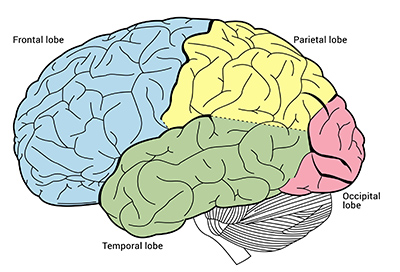
\includegraphics[width=0.5\linewidth]{images/BrainLobes.jpg}
        \caption{The brain's four external lobes \cite{LobesOfBrain}}
        \label{fig:external-lobes}
    \end{figure}

    Although most brain functions require an interplay of many different regions across the entire brain, each lobe can still be made responsible for the bulk of certain functions \cite{LobesOfBrain}. The individual lobes therefore can be associated with the following:
    %
    \begin{description}
    \item[Frontal lobe:] Executive functions like planning, reasoning, and problem-solving. But it is also involved in emotional regulation and what makes up the personality.
    \item[Parietal lobe:] Integration of sensory information, which includes taste, touch, temperature, and pain. Also associates visual and auditory signals with memories.
    \item[Occipital lobe:] Decoding of visual information into form color and movement. Facilitates visual identification of Objects.
    \item[Temporal lobe:] Analyses auditory information and makes it possible to distinguish volume and frequency of sounds.
    \cite{thebrain-SimpleToComplex-neuroAnatomy-b}
    \end{description} 
    
    % If useful/necessary, elaborate on Cerbellum here
    
    Only when a sagittal section of the brain is made (which is a cut through the brain that separates the two hemispheres), do many more important structures become visible. For example the cingulate gyrus, as well as other parts of the limbic system \cite{thebrain-SimpleToComplex-neuroAnatomy-i}.
    
    \begin{figure}[H]
        \centering
        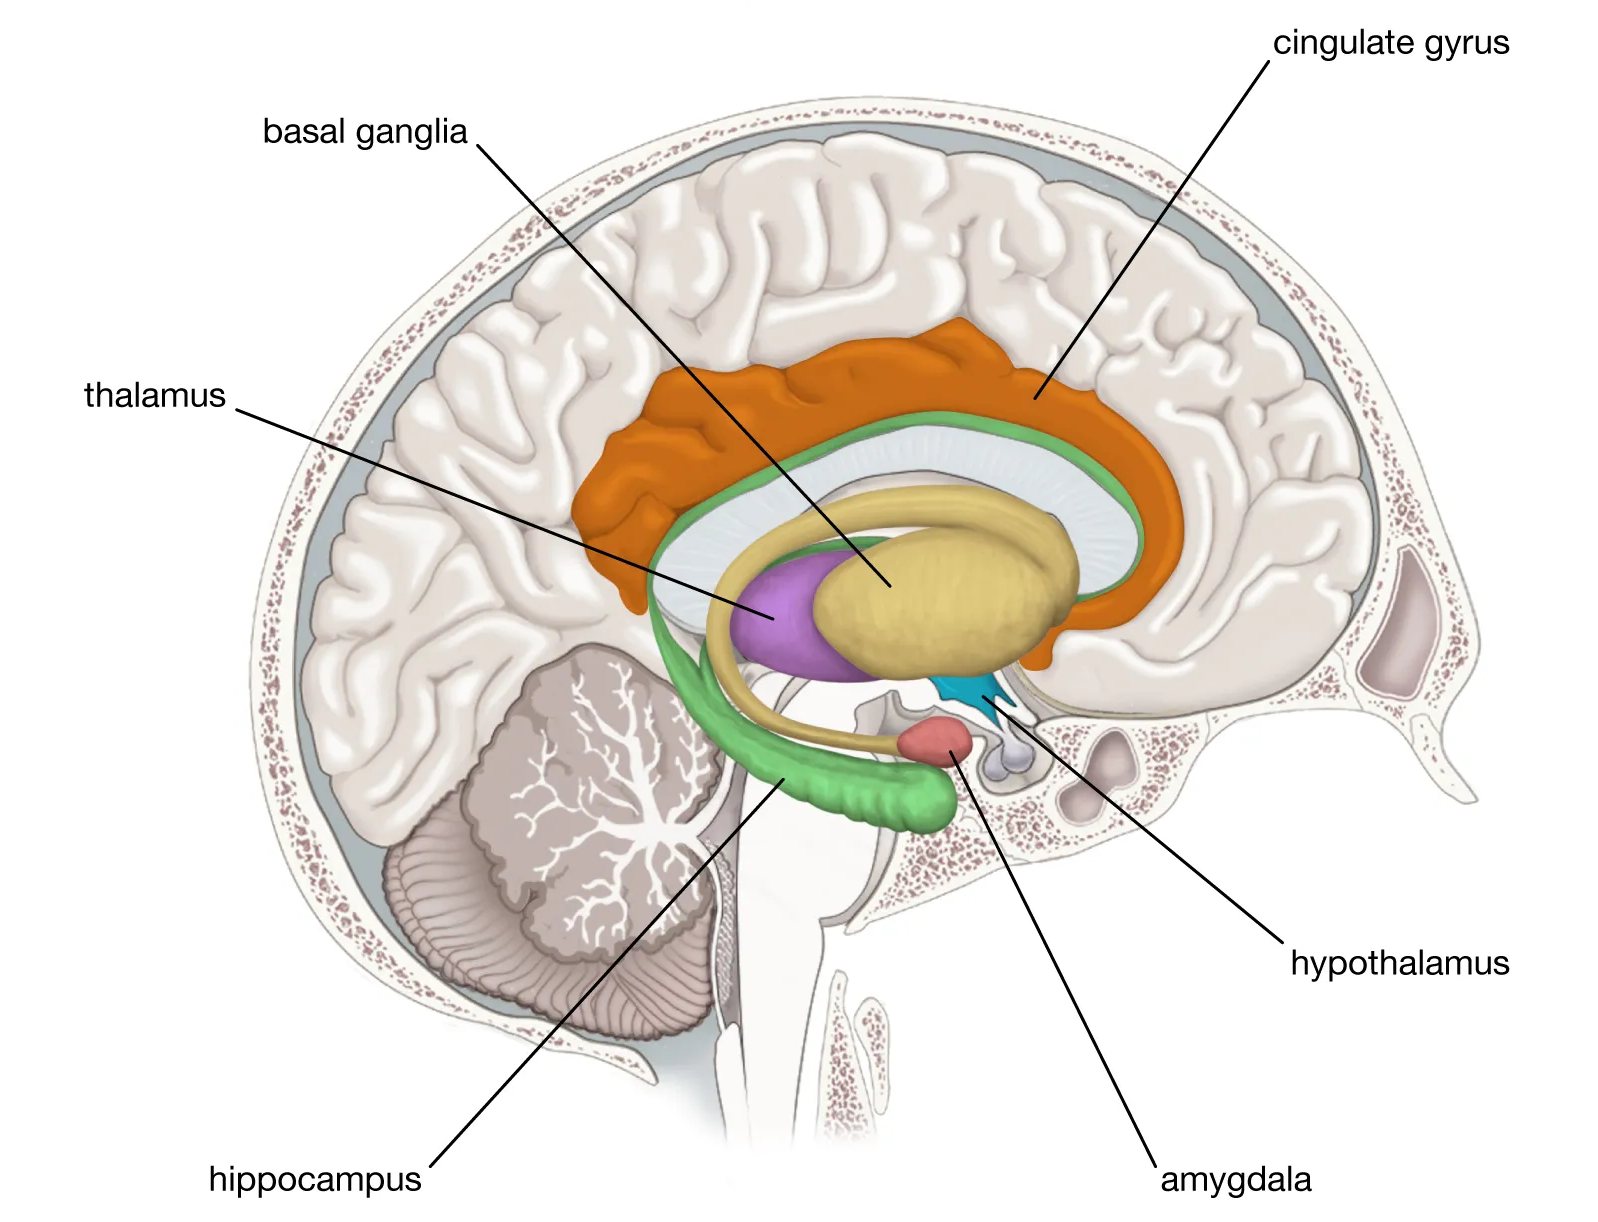
\includegraphics[width=0.5\linewidth]{images/brain-limbic-system-cut.png}
        \caption{Primary components of the limbic system (\cite{LimbicSystem} - modified)}
        \label{fig:limbic-system}
    \end{figure}

    Due to its high interconnectedness with other parts of the brain, there is no overall agreement on every component of the limbic system. Nonetheless, the structures depicted above can be considered its primary components. As a whole, it is involved in emotional responses, olfaction, and motivation but also the formation of long-term memory \cite{LimbicSystem}.

    % possible elaboration of more specific brain structures, that are related to the cognitive processes i am going to research

    Taking a look at the basic functionality of the brain and how it processes information, we encounter two very different aspects of its signal propagation. Whilst one is composed of direct and precise wiring between neurons, the other one is way more diffuse and based on a broader modulation of signals. \\
    The brain's wiring is established with the help of axons, which are an extension of a neuron that propagates a signal to its connected neurons. They enable fast and precise communication between various parts of the brain. Circuits that are formed like this, make complex processes possible and allow for essential information exchange. For example, our emotional limbic system and the rational cortex are connected like this and therefore can maintain a constant dialogue to integrate their desires \cite{thebrain-SimpleToComplex-neuroFunction-b}.

    %elaboration on hormonal brain?


\subsection{Neurons and Glial Cells}
%Cellular Organisation:
    % Neuron Anatomy
    The human nervous system allows us to respond to internal and external stimuli and comprises two types of cells. Neurons are the ones that transmit information with the help of electrical and chemical signals. Glial cells on the other hand act in a supportive manner. \\
    \textbf{Neurons} consist of the usual cell body but also show two additional parts: dendrites and an axon. Both play an important role in the transmission of information. Dendrites exhibit a tree-like structure, which is responsible for receiving input from other cells. The Axon is the extension of the cell that transports signals outwards. The length of these axons can vary by a lot. Whilst some only connect to other neurons in the brain and therefore are fairly short, others stimulate muscles over a long distance. But not only does the length of the axon differ between neurons. Depending on their role in the nervous system, they can take on many different shapes and sizes (Figure \ref{fig:neuron-types}) \cite{Banich.2018}.
    
    \begin{figure}[H]
        \centering
        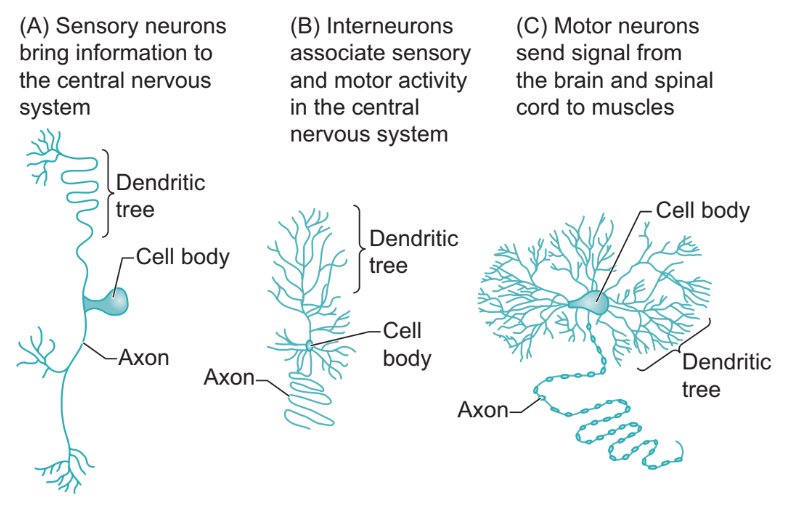
\includegraphics[width=0.75\linewidth]{images/neuron-types.png}
        \caption{Common examples of neurons \cite{Banich.2018}}
        \label{fig:neuron-types}
    \end{figure}

    
    % Glial Cells' anatomical role
    There exist different types of \textbf{Glial cells}, which all play an important role in intercellular communication. Even though their involvement might be a bit less obvious than that of neurons, they are just as essential for our nervous system. In fact, without them, the transmission of information via the neurons, would not even be possible \cite{Banich.2018}. 
        % Different types and their function, briefly mention role of axon myelination
        The following glial cells support the functioning of the central nervous system:
        \begin{description}
            \item[Astrocytes:] They take on the most complex functionalities of glial cells, which range from supplying mechanical support to maintaining and cleaning the extracellular environment \cite{thebrain-SimpleToComplex-cellularFunction-i}. But most importantly they provide neurons with nutrients. Via a connection to the capillaries in the Brain, they let glucose enter into their cell, partially metabolize it, and pass it on to the neurons \cite{thebrain-SimpleToComplex-cellularFunction-a}.
            \item[Microglial cells:] This type of glial cell acts protectively, as a primary defense mechanism against invaders. Therefore they can be considered the macrophages of the brain. 
            \item[Oligodendrocytes:] These cells provide a unique structural support, by wrapping around the axons of numerous neurons. Doing so in a very specific way, they create a myelin sheath that allows for accelerated conduction of nerve impulses \cite{thebrain-SimpleToComplex-cellularFunction-i}
        \end{description}

    
    % Neuronal Functions: specifics on how action potentials work
    Only when all these structures of different neurons and glial cells work together, can our brain function properly. Everything we experience, like thoughts, emotions, and the ability to move, is based on the capability of individual neurons to communicate.
    
        % Electrical properties, thresholds, place of summation and electrical conduction
        Taking a closer look at how this communication takes place, two complementary processes become apparent. One is the \textbf{chemical transmission} of signals which can be found between two neurons, at the synapse. Here chemical messenger molecules are transferred from the sending neuron to the receiving side. Details regarding this process will be covered in a later subsection dedicated to the synapse and molecular processes in the brain. \\
        When a signal arrives at another neuron, an electrical impulse arises. This impulse is then propagated inside the neuron via the other process, called \textbf{electrical conduction} \cite{thebrain-SimpleToComplex-cellularFunction-b}.
        % Relate to information value (all or nothing, frequency relevant)
        The dendrites of a single neuron receive impulses from thousands of other neurons. These impulses can either be excitatory (meaning they increase the probability of triggering a new impulse in the neuron) or inhibitory (when they reduce this probability). Depending on the type of impulse, a small potential is generated inside the neuron, which is positive for excitatory ones and negative otherwise. With the help of passive diffusion, this potential is propagated toward the cell body, losing intensity the further it travels. At the beginning of the axon, a summation of all impulses takes place. Only when the neuron's excitatory threshold is exceeded, a new impulse is generated and sent down the axon. In contrast to the passive diffusion, this so-called \textit{action potential} propagates actively with a maintained signal strength \cite{thebrain-SimpleToComplex-cellularFunction-i}. \\
        \textbf{Action potentials} are an "all or nothing" signal, meaning they do not vary in amplitude or intensity. Regardless of how far the neuron's threshold is exceeded, it will always result in the same signal. Therefore, a neuron can only transmit information by varying how many action potentials it generates per second. An action potential is propagated extremely fast and at any given point of the axon, it will not last longer than a few milliseconds. After it passes, the axon membrane exhibits a short refractory period, during which it cannot be stimulated. This also prevents the signal from being propagated in the wrong direction \cite{thebrain-SimpleToComplex-cellularFunction-a}

        % image action potential?
        
    % Myelination in detail
    To enable such a rapid propagation of the nerve impulses, many axons are wrapped inside an insulating sheath. This \textbf{myelin sheath} consists of a fatty substance and is formed with the assistance of glial cells. Within the brain, oligodendrocytes take on this task by wrapping their cell membrane around the axons.
        % nodes of Ranvier, place of ion channels
        But this sheath does not envelop the entire length of an axon, leaving gaps called \textit{nodes of Ranvier}. These nodes, spaced from 0.2 to 2 millimeters apart, facilitate a special conduction mechanism. Action potentials only have to leap from one node to the next, where the ion exchanges occur that regenerate the signal. In contrast to the continuous propagation of non-myelinated axons, this "saltatory conduction" is more efficient and much faster \cite{thebrain-SimpleToComplex-cellularFunction-i}.

 

\subsection{Synapses and Ion Channels}
%Molecular Organisation: 
    % Synaps Anatomy
    The place where an axon, connects to the dendrites of another neuron, is called a synapse. 
        % Electrical and Chemical
        Generally, there are two different types of synapses. One is the \textbf{electrical synapse}, where the cells touch physically and are connected by minuscule openings, that allow for a direct transmission of nerve impulses between them. Secondly, via \textbf{chemical synapses}, where the neurons remain separated and specific molecules have to traverse the gap to transmit the nerve impulse.
        While electrical synapses facilitate a swift transmission, chemical synapses are comparatively slower yet offer significantly more flexibility. This flexibility is fundamental to the process of learning \cite{thebrain-SimpleToComplex-mollecularAnatomy-b}. \\
        % Chemical Synaps in depth
        % Neurotransmitters (excitatory, inhibitory)
        The basic anatomical structure of such a chemical synapse can be seen in Figure \ref{fig:synapse} and facilitates the signal transmission as follows:
        % Function of Synaptic transmission (and role ion channels)
        When an action potential of the presynaptic neuron arrives at the terminal bouton (or axon terminal), the electrical signal is transformed into a chemical one. This happens with the help of synaptic vesicles, which contain neurotransmitters. These vesicles are waiting inside the terminal bouton and fuse with its membrane upon arrival of the action potential. Consequently, many molecules of neurotransmitters are released into the \textit{synaptic cleft}, which describes the gap between the pre- and postsynaptic neuron. When they reach the other side, they bind to receptors which are embedded into the membrane of the postsynaptic neuron. Receptors are proteins that change their configuration in response to the binding of a neurotransmitter and therefore the electrical charge of its neuron. They do so by influencing the ion flow across the membrane. Whether this results in an excitatory or inhibitory potential, depends on the receptor \cite{Banich.2018}.
        
        \begin{figure}[H]
            \centering
            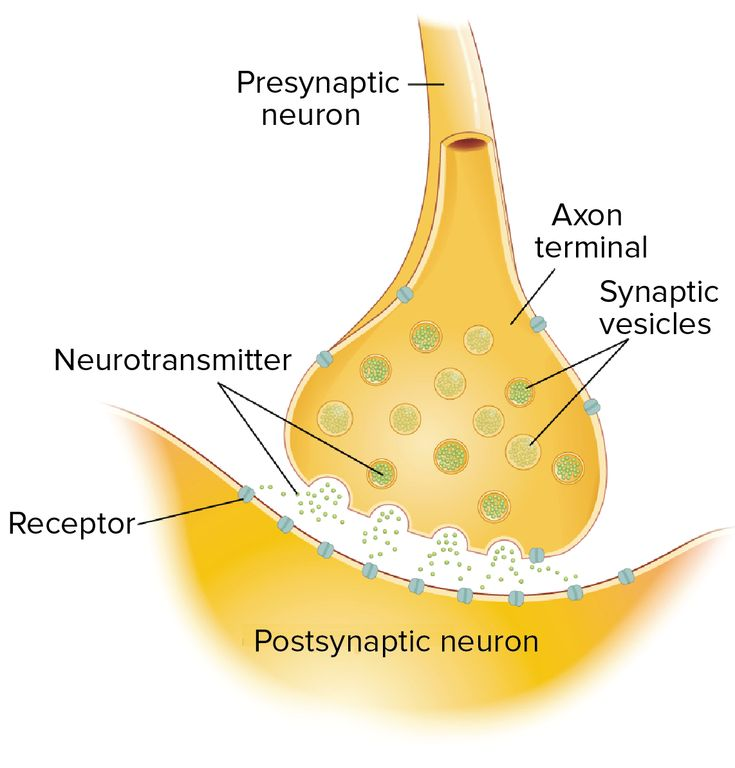
\includegraphics[width=0.5\linewidth]{images/synapse.jpg}
            \caption{Basic anatomy of chemical synapse}
            \label{fig:synapse}
        \end{figure}
        
    % Ion Channels and Nerve Conduction in Axon
    Any nerve impulse propagated inside our neurons, is simply the movement of electrically charged molecules (also known as ions) across the neural membrane. But without specialized \textbf{ion channels} in the membrane that coordinate this movement, something complex like our self-awareness would never be possible. Therefore, our brain relies heavily on these channels, consisting of large proteins. On a fundamental level, they give the neuron membrane a semi-permeable property, meaning that some ions may traverse it more easily than others. This semi-permeability controls, how the charged molecules distribute themselves across the membrane. In a resting state, an equilibrium is reached where the charge inside of the neuron is more negative than outside \cite{thebrain-SimpleToComplex-mollecularFunction-i}. %Resulting in a resting potential of about -70 millivolts.
    \\
    Should this equilibrium be disturbed and a strong enough depolarizing stimulus arise at the beginning of an axon, the ion channels are also responsible for \textit{producing the action potential}. By allowing many positively charged sodium ions to enter the cell, a strong depolarization happens and for a moment, the cell's charge even becomes more positive than outside. Then the channels of other positively charged potassium ions open, so they can leave the cell, and the ones of sodium close again. This leads to a strong hyperpolarization, such that the relative charge becomes even more negative than in the beginning. After the potassium channels close as well, the neuron slowly re-assumes its equilibrium and resting potential \cite{Banich.2018}.
    This sequence takes place at one node of Ranvier after the other, which is how the action potential is propagated to the end of the axon.
    


\section{Cognitive Processes}
    
    % Introduction to the General topic
        % What are coginitve processes
        % which ones am i presenting
    Cognitive processing refers to a series of activities involved in creating and managing mental representations of information. Cognitive processes encompass for example: attention, perception, reasoning, learning, but also the expression of emotions and more.
    They can occur consciously, such as when learning a concept, or unconsciously, as in skill acquisition. Further, they may be internally generated, like when recalling a memory or prompted by new sensory input from the environment, such as when navigating a maze \cite{Krch.2011}.
    % Create logical integration of section into thesis and a short overview
    % Specifically, the perception of emotions like fear and anxiety, are of special interest in the context of this thesis. Therefore, this section explores the involved cognitive processes, including the related brain structures and their neural topology. 
    
    \subsection{Emotions - Fear and Anxiety}
        % What is Fear and Anxiety
        % What is their function
        Fear and anxiety exist in the first place to alert us of potential dangers, threats, or conflicts and prompt us to respond appropriately. While some experts see fear and anxiety as the same thing, others believe they are different experiences \cite{Steimer.2002}.
        Even though they fall into the same category of alert signals, they arise in different scenarios. Whilst fear prepares us when confronted with a known external threat, anxiety takes over in case of internal conflict or when the danger is unknown \cite{kj.1995}.
        But also if anxiety and fear are considered different emotions, they can still share similar brain and behavior patterns. Some even suggest that anxiety could simply be a more complex version of fear, helping us to adapt and prepare for what is ahead \cite{Barlow.2000}.

    \subsubsection{Related Brain Structures}
        % what structures are involved (amygdala, simple circuit)
        % how does activity in amygdala relate to fear
        
        % 0. The biology of fear - 235, 238
        There are specific brain circuits involved, when we experience emotions and research has made good progress in the last decades to identify them \cite{Steimer.2002}. The long-established assumption, that emotions like fear and anxiety originate almost entirely from the limbic system, is by now considered obsolete \cite{LeDoux.2000}. 
        Nonetheless, the \textit{amygdala} (which is part of the limbic system) plays a central role, when it comes to fear and anxiety. 
        %(Using Neuroscience) -> amygdala damage
        It has for example been shown, that people with brain damage in the area of the amygdala, do not show physical reactions to threats \cite{Phelps.2006}. 
        % 1. The biology of fear 237 -> electrical stimulation = fear
        Other studies found that the electrical stimulation of the amygdala causes a complete fear response. Specifically, the lateral and central nuclei of the amygdala have been identified to generate the strongest responses and therefore may be considered the most important \cite{panksepp.1998}. \\
        % 2. The amigdala -> anxiety related to amigdala 2.0
        But many studies have also shown that for anxiety responses as well, the amygdala is of central importance \cite{Ferry.2017}. 
            % activity of amigdala = anxiety 2.2
        \textcite{Kim.2011} have suggested, that the activity level of the amygdala, may correlate with the intensity of anxiety - even if no threat was involved. \\
        As already suggested, it is not surprising that anxiety seems to be most dependent on sub-regions of the amygdala, that are similar to those related to fear. Next to the basolateral complex and the medial nucleus, the central nucleus appears critical \cite{McDonald.1982}. This central nucleus is, based on studies with rodents, crucial for the basic defensive responses, that are triggered by fear \cite{Davis.2001}.
        
        
    \subsubsection{Neural Topology and Molecular Mechanisms}
    
        % how are the Neurons connected there?
            % different structure of subnuclei - The Amygdala 2.1
            All the above-mentioned nuclei of the Amygdala, exhibit differences in their cell types, but also when it comes to connectivity and functional organization \cite{McDonald.1982}.
            % central nucleus essential
            Since the \textit{central nucleus} seems to be the part of the amygdala, that correlates the strongest with fear and anxiety, it would pose an interesting structure to simulate the cognitive process. 
            
        % what neurotransmitters are involved?
            Many neurotransmitters and other neuromodulators are involved in fear and anxiety \cite{Steimer.2002}. Amongst these, \textit{GABA} plays an important role. With its inhibitory function, it can help to calm the neuronal hyperactivity that is associated with anxiety \cite{thebrain-emotions-mollecular-a}.
        

    \subsection{Learning and Memory} 
    % Psychological
    % Very top-level definition of learning and Memory and how it works
    % differentiation short/long term memory - functionally
    Learning allows us to hold on to information, emotions, and impressions that can shape our behavior. It is the brain's primary function, wherein it constantly adapts its structure to better represent our experiences. This leads to memory, the lasting presence of personal experiences and general knowledge.
    Such memories are based on our perception of things and connect the information about different aspects, processed across our brain.\\
    Different forms of memory can be distinguished. \textit{Short-term memory} for example, allows for the retention of information for not more than a minute and is created based on what sensory inputs were paid attention to. An extension of this concept is the \textit{Working memory}, which facilitates cognitive operations on temporarily stored information, like reasoning, performing computations, or recalling a recently heard list.\\ 
    \textit{Long-term memory} on the other hand, describes any memory that is maintained over a longer period. It includes memories that are consolidated to different degrees and therefore can be recalled from days to years later \cite{thebrain-memory-psychological-a}.

    \subsubsection{Related Brain Structures}
    % Neurological
    % Focus on the Hippocampus and its role
    % importance of Short wave ripples and theta nested gamma oscillations
    Regarding short-term and working memory, the prefrontal cortex plays a fundamental role. It merges the information stored across other parts of the cortex and allows for its retrieval and reasoning \cite{thebrain-memory-neurological-a}. But also the hippocampus and certain activity patterns there, are involved in working memory. \textcite{Axmacher.2010} suggest that certain rhythms produced by the hippocampus can be associated with working memory performance. Specifically, the coupling of theta (4-8 Hz) and gamma (25-100Hz) rhythms (so-called \textit{theta-nested gamma oscillations} \cite{Aussel.2018}), seem to be of importance.\\
    However, especially for consolidating memories and their transition into longer-term memory, the hippocampus plays a crucial role. It is responsible for the formation of new associations between different areas of the cortex. For example, connecting the music heard with the faces seen at a party, to form a memory of it. Whether such associations then are reinforced until they turn into long-term memory, can depend on different factors. One important being their emotional relevance, which is evaluated in cooperation with other parts of the limbic system \cite{thebrain-memory-neurological-a}. Relevant patterns and associations, that were made during the day, are further strengthened via the occurrence of high-frequency oscillations during sleep. These particular oscillations, which are also called \textit{sharp wave ripples} (SWRs), mimic the patterns in a temporally compressed manner and therefore enhance synaptic plasticity and memory consolidation \cite{Girardeau.2011}. As a certain association strength is reached, the associations become encoded in the cortex and the hippocampus stops being involved \cite{thebrain-memory-neurological-a}.
    
    \subsubsection{Neural Topology and Molecular Mechanisms}
    % Cellular, Molecular
    % Focus on cells of Simulation (Acetylcholine?)
    The hippocampus proper is made up of three major sub-areas, called the CA1, CA2, and CA3. These in turn consist for the most part of pyramidal neurons. Input comes from the entorhinal cortex (EC) via the dentate gyrus (DG), is then processed in the hippocampus proper, and sent out from the CA1 to the subiculum \cite{thebrain-memory-Cellular-a}.
    
    % Insert graphic of hippocampus anatomy

    On a molecular level, learning is facilitated by Long-term potentiation, which is a mechanism that allows the strengthening of synapses. This is usually triggered by a short but high-frequency stimulation of the presynaptic neuron, which leads to a stronger (higher amplitude) response of the postsynaptic one. This change in amplitude appears due to a series of processes, including the creation and efficiency increase of certain ion channels at the postsynaptic neuron \cite{thebrain-memory-molecular-a}.

    
\section{Cognitive Warfare}

    % Why is it necessary to elaborate on the topic and how am I going to do this (what is the structure and content of this subsection)
    \textit{Cognitive warfare} is a term for an emerging form of warfare, which encompasses a broad field of practices \cite{Backes.2019} \cite{Claverie.2022} \cite{EADS.2023} \cite{MAKSYMENKO.2023} \cite{McCreight.2024} \cite{Miller.2023}. This section explores some of its definitions and suggests a way of categorizing them. Furthermore, the category that is relevant for this thesis, is identified and described in more detail before the general relevance of the topic is pointed out.


    \subsection{Categorization of Cognitive Warfare}

        % What is Cognitive warfare (broad definition, mention different ones)
            % ref: CW-russian threat, cognitive warfare ethical analysis, the cw concept
        A range of definitions for \textit{cognitive warfare} can be found in the literature, which describe varying scopes and aspects of it. \textcite{Claverie.2022} for example take a very general stance when they define cognitive warfare as "the art of using technological tools to alter the cognition of human targets" \cite{Claverie.2022}. This leaves both the method and exact effects on cognition open and therefore encapsulates most associations with the term.
        Other literature defines it more specifically as "altering through information means how a target population thinks, and through that, how they act" \cite{Backes.2019} or points out the involvement of "technologies capable of influencing or controlling cognitive functions and emotional states" \cite{EADS.2023}.
        
        % What Forms exist (focus on electro-magnetic attacks)
        These more specific definitions already characterize two major forms that can be identified. One is the more established one, covered by \textcite{Backes.2019}, where \textbf{information} and knowledge are the main focus. With the help of propaganda and disinformation, the beliefs of large populations are manipulated in the hope of influencing their choices and behavior. \\
        The other form is characterized by advanced \textbf{technologies} and their more fundamental influence on cognition and mind. Attacks performed with such technologies can be labeled as \textit{NeuroStrikes}, and employ for example so-called "Soft-Kill Radio Waves" which essentially are a form of EMR. They can cause significant cognitive damage and interfere with their targets' brain function \cite{EADS.2023}. This thesis focuses on the latter form of cognitive warfare.

        
    \subsection{NeuroStrikes and the Havana Syndrome}
    
        Since NeuroStrikes are the relevant form of cognitive warfare for this thesis, their effects and underlying technology shall be explored in more depth. In this context, the \textit{Havana Syndrome} serves as an important reference, as it is the best-documented collection of potential NeuroStrike incidents. 
        
        The \textbf{Havana Syndrome} describes a condition, that was coined by a collection of health incidents, which were distinct from any previously documented, neurological, or mental disorder \cite{Pavlin.2020} \cite{Bartholomew.2024}. It occurred first in Havana in 2016, when an individual who was assigned to the U.S. embassy, suddenly suffered from acute pain, coupled with a loud noise and cognitive impairments, followed by a range of long-term symptoms. Similar cases arose over the following years, while a closer investigation was not performed until 2020 when the National Academy of Sciences published an extensive report. Even though the assessment was difficult, due to a lack of complete and uniform clinical data, it was suggested that the most probable source for the symptoms was a form of NeuroStrike (directed, pulsed \textit{Radio Frequency} (RF) energy). Other potential mechanisms, like chemical or infectious agents, were deemed highly unlikely or in the case of psychological and social factors, could not explain the whole picture \cite{Pavlin.2020}. Even though it has to be stated that this topic is still debated and contradicting arguments exist \cite{Bartholomew.2024}, most literature on the technical form of cognitive warfare considers this syndrome to be related to it \cite{EADS.2023} \cite{McCreight.2022} \cite{McCreight.2024}.

        Based on that, pulsed RF EMR certainly represents a relevant form of NeuroStrikes, which could be responsible for the impairment of a series of cognitive processes. Its exact effects on the brain and how they could be mitigated are the subject of this work.
        

    \subsection{Relevance}
        % active developments
        Many countries and institutions are already applying cognitive warfare to such a degree, that its importance should not be underestimated \cite{Claverie.2022}. Whilst there are several reports of Russia, practicing cognitive warfare in its information-based form to influence elections \cite{Backes.2019} and during times of war \cite{MAKSYMENKO.2023}, there also exist incidents that are associated with NeuroStrikes (as described in the previous subsection). Furthermore, the Chinese communist party is reportedly investigating technologies related to these attacks \cite{McCreight.2024} and even has a dedicated military program in place to develop weapons for this purpose \cite{EADS.2023}.
        
        % passive threat
        But regardless of the intentional and active developments of such attacks, it has to be recognized that even neuroscience research performed with good intentions and health improvements in mind, may be misused for harmful military purposes \cite{McCreight.2024}. Consequently, the threat imposed by these technologies and cognitive warfare of this form is already very real and will only become larger over time and with advancing research.



\section{Brain-Computer Interfaces}
    % General description of what brain interfaces are: gateway between brain and computer
        % reading brain signals (Nicolas)
        % stimulating brain (William)
        % Uni and Bidirectional (Rao.2019)
    Brain-Computer Interfaces are systems, that enable information transfer between the brain and a Computer. This encompasses technologies that allow for the sensing and interpretation of brain activity \cite{NicolasAlonso.2012}, as well as ones that enable neural stimulation \cite{WilliamJ.Tyler.2017}. These two technologies may also be combined to create a bidirectional system \cite{Rao.2019}.\\
    BCIs enable users to engage with their environment independently of peripheral nerves and muscles. They create a novel pathway, that translates their intentions into signals, which may control many devices like computers or prostheses. This enables for example people who are "locked in" or severely disabled, to communicate or regain other fundamental capabilities. It therefore is of especially high interest to those groups. However, BCIs also have potential use cases in non-medical environments like entertainment \cite{NicolasAlonso.2012}.
    
    % general sensing methods
    When measuring brain activity, for example, to interpret the users' intentions, there are generally two phenomena that can be observed. One is the \textit{electrophysiological} activity of the brain and the other consists of its \textit{hemodynamics} \cite{NicolasAlonso.2012}. \\
    The \textbf{electrophysiological} activity stems from the currents that arise during the propagation of action potentials and therefore is directly related to information processing \cite{Baillet.2001}.
    \textbf{Hemodynamic} changes, on the other hand, can be traced back to the fact that active neurons are supplied with more glucose and oxygen than inactive neurons. This leads to more oxyhemoglobin in the active areas and allows for a distinction from nonactive ones by observing the local oxyhemoglobin to deoxyhemoglobin ratios \cite{Laureys.2014}. This therefore is only indirectly related to the processing of information.
    
    % Invasive - non Invasive (8 reasons, WilliamJ)
    Many different detection and stimulation methods are used in BCIs, which may be categorized according to their level of invasiveness \cite{Bernal.2023}. In the following section, the differences between the two, as well as some specific examples are discussed.
        

    \subsection{Non-Invasive Brain Interfaces}
        Non-invasive methods have the inherent benefit of being applicable without prior surgery. Instead of implanting an electrode into the user's brain, they act outside of the skull \cite{WilliamJ.Tyler.2017}. Even though this means that they are limited to recording activity with lower resolution \cite{Lebedev.2006}, they certainly are the preferred choice for short-term usage scenarios \cite{Luan.2014}. \\
        % Measuring brain activity -> brain computer interfaces, a review
        The following are examples of such non-invasive methods.
        
        \subsubsection{Recording Methods}
        \begin{description}
            \item[Electroencephalography (EEG)] is a method that records the electrophysiological activity, being especially sensitive to the extracellular currents that come with it \cite{Baillet.2001}. Since it only requires electrodes to be placed on the scalp for measurements, it is a very easy and popular method. However, a major downside is the poor signal quality, which suffers from a lot of background noise.
            \item[Functional Magnetic Resonance Imaging (fMRI)] detects hemodynamic changes, like local blood volumes and flows, as well as oxygenation levels. It does so with the help of MRI scanners that create electromagnetic fields. This results in spaciously very accurate readings, that can be used to identify precisely which brain regions are active \cite{deCharms.2004}.
        \end{description}

        % Stimulating brain -> WilliamJ.Tyler.2017
        \subsubsection{Stimulation Methods}
        \begin{description}
            \item[Transcutaneous Electrical Neurostimulation (TENS)] is the broadest category of methods, to stimulate the brain non-invasively. The basic procedure constitutes the transmission of electrical current (which can be static or dynamic), via electrodes that are placed on the skin, to nerves. The applied current then modulates neuronal activity directly. Even though it is a complicated procedure to control which neurons are activated, this method can be very effective. It might even be possible to achieve drug-like outcomes with reduced side effects or augmenting cognitive performance \cite{WilliamJ.Tyler.2017}. 
            \item[Ultrasonic Neuromodulation (UNMOD)] is a unique method, which has been shown to allow, if applied in a pulsed manner, to stimulate neuron activity. Interestingly, it may do so via mechanical mechanisms of certain ion channels instead of influencing the electric charge directly \cite{Tyler.2008}. But the field of this methodology is still somewhat new and it will take time to create a deeper understanding of the mechanical influences on our brain activity. Nonetheless, it holds loads of potential for future development \cite{WilliamJ.Tyler.2017}.
        \end{description}


    \subsection{Invasive Brain Interfaces}
        % benefits compared to Non invasive
        Even though non-invasive interfaces are a great choice for many applications, there are scenarios where their limited precision is insufficient. For example, most researchers agree that without invasive methods, exercising control with multiple degrees of freedom over prostheses is impossible \cite{Lebedev.2006}. However as these invasive methods require the implantation of electrodes inside the skull, their application bears substantial health risks, that have to be addressed to make them a viable option \cite{Kennedy.2000}. \\
        % Measuring -> brain-computer interfaces, a review
        Some examples of such invasive methods are presented below.

        \subsubsection{Recording Methods}
        \begin{description}
            \item[Electrocorticography (ECoG)] is a method, where electrodes are placed on the brain surface, to record its electrical activity. It, therefore, follows a similar approach to EEG whilst being closer to the activity and avoiding the skull as an obstacle. Consequently, it achieves a higher spatial and temporal measurement resolution and is less susceptible to noise \cite{Ball.2009}. Advanced versions of this method, make it already possible for their users to control a cursor in two dimensions \cite{Schalk.2007}.
            \item[Intracortical Neuron Recording] is a technique, where electrodes are not placed outside, but rather inside the brain. Specifically into the cortex, where it measures the electrophysiological activity of neurons \cite{NicolasAlonso.2012}. Besides achieving a significantly higher resolution than non-invasive alternatives and providing easier-to-interpret signals, their quality can degrade over time. This can happen due to issues with cerebral tissue reacting to the electrodes \cite{Polikov.2005}.
        \end{description}
        % Stimulating
            % DBS (deep brain stimulations) -> 8 reasons
        \subsubsection{Stimulation Methods}
        \begin{description}
            \item[Intracortical Microstimulation (ICMS)] is a technique, that focuses on the stimulation of the cortex \cite{Vidal.2016}. It has demonstrated significant utility in comprehending the functions of cortical activity and enables the manipulation of sensory perceptions through brain stimulation. This simulation of sensory input has the potential to restore functional vision \cite{Zhao.2023} and could also be used to supplement prostheses with tactile perception and thereby improve the performance with it \cite{Flesher.2021}.
            \item[Deep Brain Stimulation (DBS)] is a method that comprises the stimulation of structures, that lie deep inside the brain and has been applied since the late 20th century. It delivers continuous stimuli, which can be adjusted in frequency and amplitude. This turned out to be useful for many different pathological situations, where it for example is applied to treat Parkinson's disease \cite{Benabid.2003}.
        \end{description}


    \subsection{Safety and Security}
    % Connection to previous BCI part (a lot of technologies that can be used in many beneficial ways...)
        % With increasing employment come also risks
            % Cyberattacks
                    % Information cycle -> Security in BCI's ?
    As presented above, there exist many different methods and technologies in the field of BCIs, which allow for a broad field of applications. And even though, the field is maturing \cite{Summerer.2009} and gaining a lot of popularity \cite{Bernal.2023}, there is not much work regarding the context of safety and security \cite{Brocal.2023}. However, BCIs bare the potential to be both, a source of risk \cite{Bernal.2021}, and a technology for risk prevention \cite{Liu.2015}. In the following, some examples of this will be discussed, before the role of BCIs in the context of this thesis is specified. 

    As \textcite{Bernal.2023} have shown, cyberattacks are an important example, of how BCIs can be a source of risk, by exploiting vulnerabilities of the technology. They pose the threat of private user information being stolen, or even the neural activity of the user manipulated \cite{Backes.2019}. Very alarming are therefore the findings by \textcite{Bernal.2021}, who analyzed and evaluated a large variety of attacks on different aspects of BCI technology. They found that even basic attacks may have a considerable impact on the safety of the user, which is especially problematic in the context that security measures for BCIs are still immature.\\
    % but they can also be used to grant safety
        % Risk identification
        % fatique detection
        % and potentially as protective measures against attacks
            % to be evaluated
    But as a collection of work shows, there also exist different approaches employing the technology of BCIs to reduce risks and improve the user's safety. This can for example be achieved by fatigue detection, which has been especially well explored \cite{Backes.2019}. As the mental state and fatigue have a significant impact on driving safety, systems like the one proposed by \textcite{Liu.2015}, can help to identify and avoid problematic conditions of the user during driving tasks.
    
    Mitigation technologies, like the ones explored in this work, may also qualify as a form of risk-reducing application. However, it is the subject of this research to show, how suited BCIs are to protect their users from the impact of electromagnetic attacks and how a protective system may be realized.
    

\section{Brain Simulations}
    Since the research of this thesis is in large parts performed with the help of simulations, this section provides an overview of the field. First elaborating on the topic and its importance in general, followed by some examples of Brain simulators.
    
    % 738 - Limited knowledge of brain
        % 741 - Until we learn
    We currently do not have a thorough understanding or an accepted theory on how the brain works on a large scale \cite{Einevoll.2019}. Even though experiments, trying to map a stimulus to its related brain activity, have been performed for quite some time \cite{Hubel.1959}, many principles of its operation remain unknown.
    % Simulations are a way to understand (even possible without?)
        % 735- still in infancy
        % 735 - cubic mil thousands of neurons
            % 736 - similar complexity as weather forecast
        % 736 - supercomputers as potential solution
    Brain simulations could help, or may even be necessary, to achieve an understanding of the wide range of mechanisms that are involved. It has to be recognized though, that the modeling of neural networks on a biological basis, is not yet a mature science. Especially due to the fact, that even representations of very small brain areas include thousands of neurons, such simulations were until recently, infeasible to compute. Although, with recent supercomputers, such limitations could be alleviated.
    % definitions:
    But before more details regarding such simulations are presented, a few terms shall be defined. Specifically, it is important to differentiate a \textit{Simulator} from a \textit{Model}. Whilst the \textit{Simulator}, describes a software tool that facilitates simulations, the \textit{Model} describes one specific collection of equations and parameters, that can be executed by such a tool (resulting in a \textit{Simulation}) \cite{Einevoll.2019}.\\
    % 739 - Models as hypothesis
        % 736 - various pros cons
    % 739 - Simulator to test hypothesis
        % Simulators usable without knowledge of every detail
    In this context, a \textit{Model} can therefore be considered as a hypothesis, of how the represented network structure might work. And with the help of a \textit{simulator}, it is therefore possible to test the hypothesis by comparing the outputs to the results of experimental findings \cite{Einevoll.2019}.\\
    In the following, a selection of simulators are presented, that are of interest for this work. An overview of potential models is then presented in the next chapter. 
        
    
    \subsection{Brian2}
    Brian2 is a simulator that works with mathematical abstractions. It allows the simulation of spiking neural networks, in an easy and efficient way, whilst maintaining a high level of flexibility. This is partly achieved, by basing its neuron models only on a set of mathematical equations. It thereby grants its users a large degree of freedom and enables them to investigate novel mechanisms without requiring a complex implementation in a low-level programming language. To increase the flexibility of the simulation process even further, it is written as a Python \cite{van1995python} library. Effectively integrating the benefits of a general-purpose programming language in the simulation environment. To still ensure fast processing of the simulation code, Brian2 makes use of runtime code generation, which transforms the simpler high-level statements, into efficient low-level code \cite{Stimberg.20.8.2019}.
    
    
    \subsection{NEURON}
    In contrary to Brain2, the NEURON simulator makes use of biologically accurate neuron models, emphasizing the realism of chemical and electrical signal transmissions, inside and across neurons. But whilst enabling the use of incredibly detailed models, the simulator leaves the choice of detail that is represented, to the creator of the model. However, it performs best in the realm of rather small and detailed networks, investigating low-level aspects like ion concentrations or membrane channel properties. It supplies a graphical interface that increases the simulator's usability, by enabling the adjustment of parameters and allowing for the representation of graphs. To investigate novel mechanisms, it provides its domain-specific modeling language NMODL, which for performance reasons is then automatically translated into C \cite{Hines.1997}. 

    
    \subsection{NEST}
    The NEST simulator employs simplified representations of neurons, that comprise few compartments at most. Therefore it is more directed toward the simulation and investigation of larger networks, instead of single neuron properties. It supplies a flexible simulation environment, that can be used with different user interfaces, including a module for Python and also a proprietary simulation language called SLI. New mechanisms can easily be added, thanks to its modular architecture, which not only allows the addition of novel neuron models but also enables the creation of simulator functions and even extensions to the simulation language itself. Regarding performance, NEST can leverage multiprocessors and computer clusters to achieve a higher simulation speed and increase memory capacity \cite{Gewaltig:NEST}.
